The aim of this thesis is to find out, how players interact with each other, while they cannot rely on direct verbal communication channels.
For this reason, a prototype of a cooperative multiplayer game is created.
For the implementation of the game, the game engine Unity\footnote{\url{https://unity.com/}}
is used. 
For the network part, the network engine Photon\footnote{\url{https://www.photonengine.com/}} is used. Photon provides an SDK called Photon PUN, which is an integration for the Unity engine.
The following sub chapters describes the game idea, how the gameplay part is implemented, as well as which and how the communication tools are implemented.



\subsection{Game idea}
\label{section:Game idea}
As the purpose of this game is the testing of communication tools, which are implemented within the game, a simple game is created.
For good cooperation, it was decided to create a cooperative multiplayer game with puzzle elements. The puzzle elements have the purpose to create cooperative puzzles, which can only be solved when players work together. There are nine levels in total the players can complete. Each level has three candies which the players need to collect. All nine levels need to be completed as fast as possible.

\subsubsection{Game elements}
\label{section:Game elements}

\begin{figure}
    \centering
    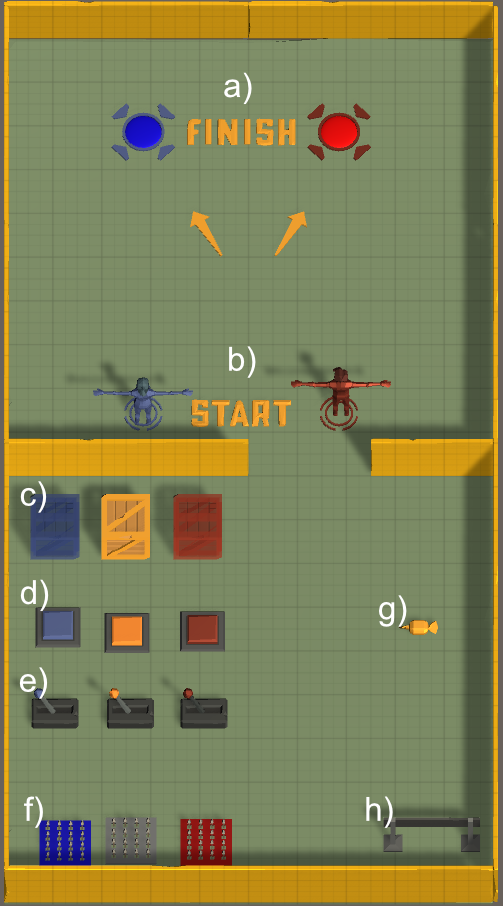
\includegraphics[scale=0.4]{images/lobby_game_elements.png}
    \caption{Overview of all game elements:
    a) goal points for each player b) start points and players c) movable boxes d) pressure plates e) switches f) traps g) candy h) barrier}
    \label{fig:game elements}
\end{figure}


Each level consists of a floor and walls. There are always two spawn-points, one for each player, as well as a goal-point for each player. The next level will load, as soon as both players are standing on their goal-point.


\begin{enumerate}
    \item Candy
    
    In each level there are three candies players are able to collect. Each candy adds one score point to the shared team score.
    \item Movable box:   
    
    The movable box blocks the way of the player. This box can be pulled towards the player or pushed in the forward direction of the player. It is not possible to move it sidewards, so the movements are limited to two directions, according to the player's position.
    \item Barrier
    
    The barrier blocks the player's path like a box. The player themself is however not able to interact with it directly. A barrier can be disabled by other elements such as switches or pressure plates
    \item Switch
    
    A switch has the purpose of enabling or disabling objects. A switch can disable a barrier, so players can pass it.
    It is also possible to enable and disable traps with it.
    
    Some switches are connected together. Both switches will only stay active, when they are activated at the same time.
    \item Pressure Plate
    
    Pressure plates are similar to switches. However, the difference to a switch is that it gets activated while a player is standing on top of it. It is also possible to move a box on top of it, so it will stay active while the both players can move around freely.
    
    There are also pressure plates that are connected with each other. Only while all connected pressure plates are active at the same time, a barrier, for example, is deactivated.
    \item Trap
    
    An active trap pulses between states of extended and retracted spikes. When the trap has retracted spikes, the player is able to move on top of it freely. When the player is on top of the spikes while they are extended, the player is sent back to the start.
\end{enumerate}

The graphics for all listed elements can be seen in Figure \ref{fig:game elements}.

Movable boxes, switches, pressure plates and traps can also have the colour of one player. 
Blue pressure plates can only be activated while the blue player or a blue box is on top of it.
Blue switches can only be activated by the blue player and only the blue player is able to move a blue box.
Even if traps are coloured, both players will respawn when they collide with it.
The same is valid for the red player and red objects

To force the player to collaborate with their partner, a blue object can only be seen by the red player, and a red object can only the seen by the blue player. As both players are not able to see every object they can interact with, they need to tell their partner, where an object is, where a box needs to be moved to and which areas they need to leave untouched.

\subsubsection{Cooperative game mechanics}
\label{Cooperative game mechanics}

To give the players the possibility to interact with each other, there are the following mechanics a player can use.

\begin{figure}[h!]
    \centering
    \begin{subfigure}[b]{0.4\linewidth}
        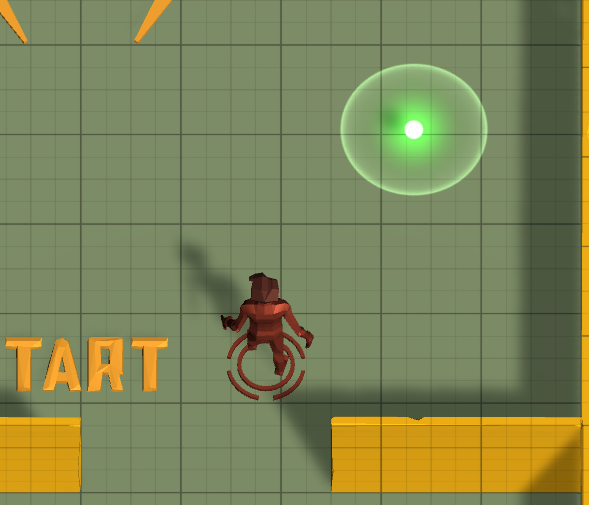
\includegraphics[width=\linewidth]{images/location_ping.png}
        \caption{Location ping}
        \label{fig:location ping}
      \end{subfigure}
    \begin{subfigure}[b]{0.4\linewidth}
        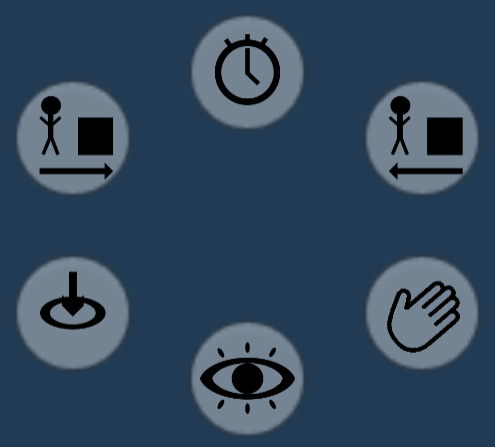
\includegraphics[width=\linewidth]{images/ping_types.png}
        \caption{All six ping types}
        \label{fig:ping types}
    \end{subfigure}
    \caption{
    Different ping indicators.}
\end{figure}

In the game, three types of pings are available. As mentioned in
Section \ref{section:Attention-focusing}, pings are counted towards attention-focusing game mechanics. With a simple left click of the mouse, a location-ping is created at the clicked position. On figure \ref{fig:location ping} a location ping can be seen.
In addition to a simple location-ping, a player can also use six semantically imbued pings. Figure \ref{fig:ping types} shows all six typed a player is able to choose. For time critical actions such as a time based switch, a countdown ping can be placed. The other five options should give the player the possibility to give commands to other players. 


\begin{figure}
    \centering
    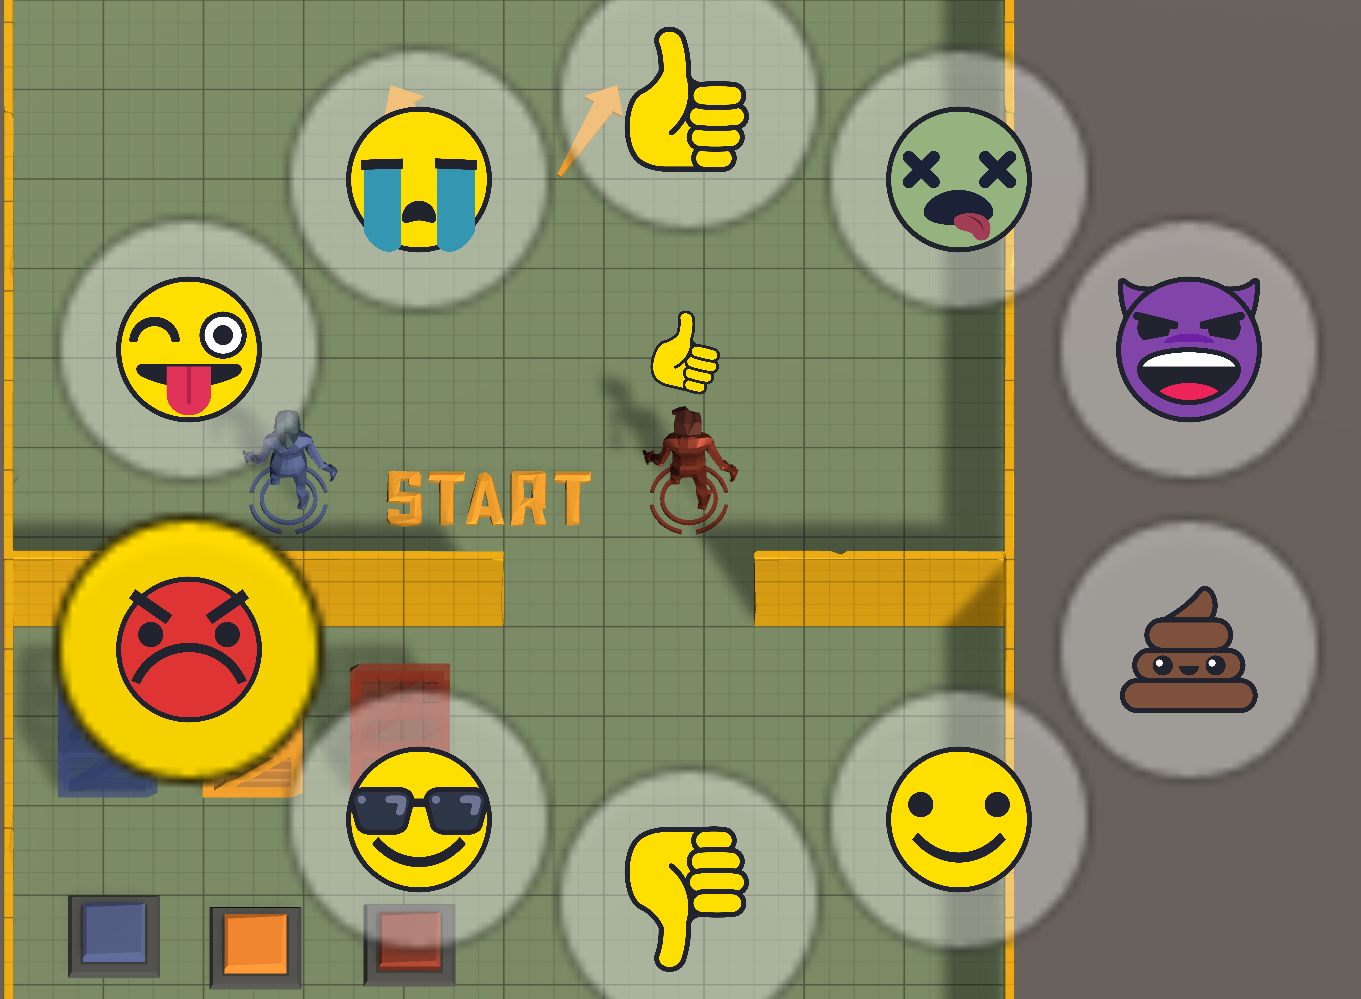
\includegraphics[width=0.5\textwidth]{images/emoji_selection.png}
    \caption{Selection interface of all emojis. A thumbs-up emoji is played above the red player.}
    \label{fig:emoji selection}
\end{figure}

For immersive communication, players get the option to use emojis.
Figure \ref{fig:emoji selection} shows all selectable emojis. The selection window opens while the right mouse button is pressed. The currently selected emoji is chosen when the right mouse button is released by the player.
In addition to all eight selectable emojis, an exclamation mark emoji can be shown above the players head. The intention behind the emojis is to give the player a way to express their feelings. Players should have the possibility to describe their current emotional state without choosing wording. This communication mechanic is a expressive emotional game mechanic as described in \ref{section:Expressive}.


\begin{figure}
    \centering
    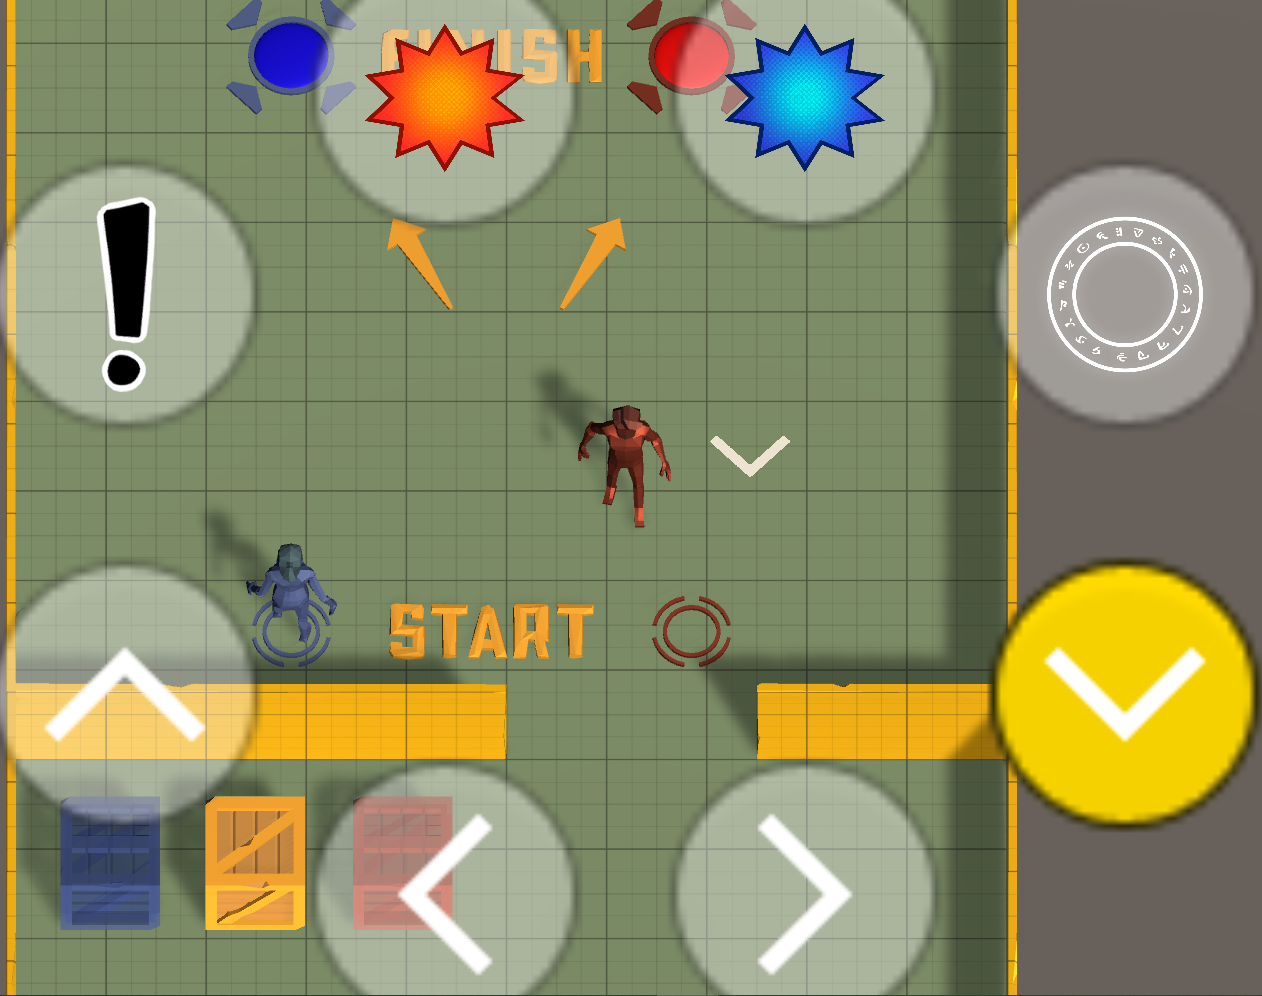
\includegraphics[width=0.5\textwidth]{images/decal_selection.png}
    \caption{Selection interface of all decals.}
    \label{fig:decal selection}
\end{figure}

To create longer lasting messages, players can create decals with eight different images, seen in \ref{fig:decal selection}. This decal-system is an environment-modifying communication mechanic, described in \ref{section:Environment-modifying}. These images are placed onto the ground below the player. Every decal overlaps the last one, but is not deleted. They last as long as the current level is played. With arrow marks on the floor as an example, players could mark a safe path which can be run along.


The fourth communication game mechanic is the recording of the current player position. While pressing the Ctrl-key or the middle mouse button, the current location of the player is saved. On release, a light transparent sphere with the player-colour is following the recorded path. This tool is not necessarily a way to communicate with each other. It was implemented to test, if players would use the ghost for emergent cooperative communication as described in section \ref{section:Emergent}. Theoretically, it could also be used to "draw" signs by walking onto the environment. The main purpose however, is to give the user the possibility to record a safe path they were able to run along.



\subsection{Gameplay implementations}
\label{section:Gameplay implementations}


\subsubsection{Player Character}

Both, the red player and the blue player, have the same scripts and components applied. They only differ by attributes like the player id, the layer to look for interactable objects, as well as the player colour.
The player input is handled via the \textit{Unity Input System\footnote{\url{https://docs.unity3d.com/Packages/com.unity.inputsystem@1.0/manual/index.html} - accessed on 14th June 2020}}. For simplicity, both player characters listen to the player input, but only the character which is controlled by the local player executes the method completly.
Each player character has a \textit{Player}-Script attached with a public method named \textit{CanUsePlayerObject()}, which returns whether the player character is controlled by the local player.

When a player joins the game, the Lobby scene gets loaded by the \textit{NetworkGameManager}. The NetworkGameManager Updates the current player map, which maps all player ids (representing the player colour) to the actor number provided by Photon. The first player is always mapped onto the red player, the second player is controlling the blue player.
The local player actor number, retrieved via \texttt{PhotonNetwork.LocalPlayer.ActorNumber}, can then be checked against the actor number behind a player id.

Per default, only the host, which here is the red player as the first player, is able to control objects. To move objects or the player around, the ownership of the object has to be transferred to the local player, who wants to modify it.
When a level is loaded, the ownership of the player characters are set to the actor number, which is mapped to the corresponding player id.

The character is then moved by the \textit{PlayerMove} script.
The input direction is saved to a corresponding variable, which is updated with an event-call, triggered by an input change. When the player is not trying to move a box, the built-in character-controller is instructed to move the player towards the wanted direction, as long there is no collision detected.
The player is also rotating towards the movement input direction.

By pressing space, the \textit{PlayerInteract}-Script checks for interactable objects in front of the player by using a raycast. If the interactable object is also moveable, which means it is a moveable box, a reference is saved.
While the \textit{PlayerMove}-Script has a reference of a \textit{MoveableObject}, it additionally moves the corresponding object. First, it is checked if the object can be moved in the given direction. When the object returns a positive call, the moveable object and the character is moved.

When the player presses the interaction-key, while a toggle is in front of the player, the \textit{Interact()}-method of the toggle is called.

The \textit{PhotonView}-Component attached to the player character synchronises the player position, rotation and the current animation state among all players.


\subsubsection{Camera}

The camera itself is handled by Unity's \textit{Cinemachine\footnote{\url{https://docs.unity3d.com/Manual/com.unity.cinemachine.html} - accessed on 14th June 2020}}-Framework.
Each scene has a virtual camera, controlled by a \textit{CinemachineVirtualCamera}-script. The local controllable player is set as the follow-target of the \textit{CinemachineVirtualCamera}-script.
Thus the virtual camera transposes the camera to a fixed offset.

\subsubsection{Overlapping Collider}

Overlapping colliders are used by pressure plates and moveable boxes.
When the OnTriggerEnter-Callback is called by Unity's physic engine, it is checked if triggers should be ignored, if the given collider should be ignored and if the overlapping object has an accepted trigger.
When the object is valid, it is added to the currently overlapping collider list. The \textit{IsOverlapping}-Method will return true, if there is a overlapping collider.
One exception exists: If the parameter is also given the player collider, and the player collider is the only collider added to the overlapping collider list, the method is returns false. This was implemented because a character was not able to pull a box object when the character was in range, while moving the object.

\subsubsection{Moveable Box}

Each moveable box has an \textit{OverlappingCollider} attached to each side , as well as a MoveableObject-Script. The \textit{IsMoveable}-Method is called by the \textit{PlayerMove}-Script, when it is set as the referenced \textit{MoveableObject}, as described before. It will return true if the overlapping collider at the required direction is returning no future collision with other objects.
When a Box is already moved by another player, the box will not be interactable until the other player stops the interaction.

\subsubsection{Pressure Plate}

Pressure plates are using an overlapping collider, which checks if there is an object above the pressure plate.
When the enabled state changes, a remote procedure call(RPC) is used to sync the pressure plate among all players.
To be able to use RPCs, a GameObject needs to have a PhotonView-Component.

As each PhotonView-Component has an id, the RPC can be sent and the correct method on the object with the same id on the other machine is called.
When the id of a \textit{PhotonView}-Component has a duplicate without the required method, an error is thrown.
This can occur when the scene has changed and the new scene has network-objects with the same id, but different scripts attached. To bypass this circumstance, Photon has the option to set the minimum id for a scene. Id's below the minimum are updated to the next free id, that is available in the current scene.

When the state is changed by an incoming RPC-Call, \textit{UnityEvent}s for enabling and disabling pressure plates are invoked. As a result, the \textit{UnityEvent} can be used in the inspector, to enable or disable objects or call public methods.

\subsubsection{Toggle}

Toggles work similar to pressure-plates but have a simple \textit{Interactable}-method, called by the PlayerInteract-Script when the player stands in front of a toggle. The state is always flipped and sent via an RPC, to synchronise all toggles.


\subsubsection{Sync-Toggle}

Sync-Toggles can only be indirectly manipulated by the player.
Sync-Toggles have elements, which can be enabled and disabled by pressure-plates or toggles. Sync-Toggles are activated when all elements are enabled. The goal-platform is a special sync-toggle which loads the next level when both players are standing on their corresponding goal-pressure plate.
When an element is enabled or disabled, an RPC is called.
The UnityEvents are only invoked when the state has changed, to prevent an RPC-loop between sync-toggles and other toggles, which are connected to each other.

Sync-Toggles can be time-critical. When not all elements are activated at the same time (with a maximum time-offset of 0.2 seconds), the elements are disabled again, which results in toggles which turn themselves off again.

\subsubsection{Traps}

Traps consist of a parent \textit{TrapCollection}-Object, which contains one or multiple Trap-objects and multiple \textit{Trap}-Objects attached to the \textit{TrapCollection}-Object.
When the trap-collection is enabled, a coroutine enables and disables all child-traps. When a player collides with the trigger of a trap, the trap will add the player to the respawn-list of the \textit{PlayerSpawnController}. This only occurs to the local player to prevent respawning because of asynchronous traps between games and network delay.


\subsection{Implemented cooperative game mechanics}
\label{section:Implemented cooperative game mechanics}

\subsubsection{UI Selection Canvas}

To give the player multiple options for pings, emojis and decals, a selection user interface is necessary. The UI is not directly bound to the game mechanics. Instead the ping, emoji and decal mechanics all use their own instance of an UI selection.
Each game mechanic can enable its corresponding UI selection canvas.

\begin{figure}
    \centering
    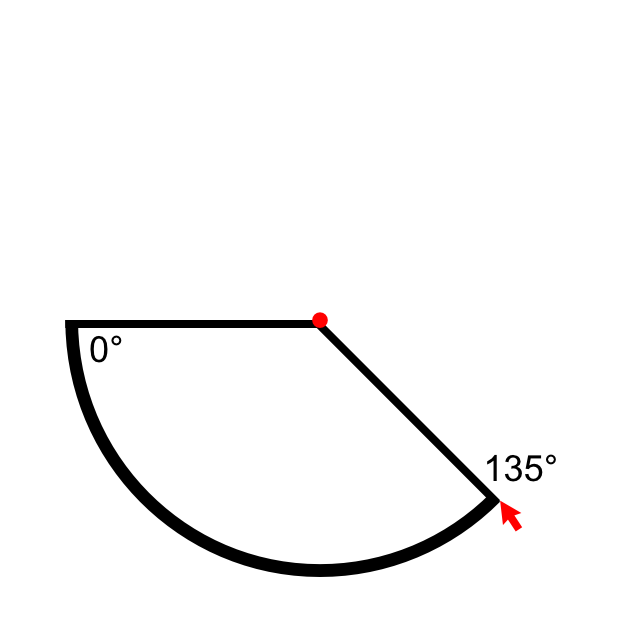
\includegraphics[width=0.5\textwidth]{images/angle_calculation.png}
    \caption{The screen angle is calculated around the centre of the screen, marked by the red dot. The red arrow symbolises the current mouse position. With these two coordinates, the screen angle is calculated using an arc-tangent function.}
    \label{fig:angle calculation}
\end{figure}

Every Canvas has a GameObject with a \textit{SelectionUI}-Component. The corresponding game mechanic implementation updates the current angle, which is used to enable the background of the selected object. The angle can be seen in Figure \ref{fig:angle calculation}. A two dimensional vector, starting from the centre of the screen to the current mouse position, is used to calculate the current screen angle in degrees.

\begin{lstlisting}[
	label=listing:Main, %for reference to this listing
	float=h,
	caption=GetScreenAngle() calculation,
	firstnumber=10
]
    private float GetScreenAngle()
    {
        var screenMiddle = new Vector2(Screen.width * 0.5f, Screen.height * 0.5f);
        var direction = this.currentMousePos - screenMiddle;
        var angle = Mathf.Atan2(direction.y, direction.x);
        angle *= Mathf.Rad2Deg;
        angle += 180;

        return angle;
    }
\end{lstlisting}

A background-GameObject is assigned to a range between two angles. The GameObject is enabled when the angle is set to a value within the range, corresponding to the GameObject.



\subsubsection{Ping implementation}

To place a ping, a raycast from the camera towards the clicked object is created, by using a ray from the camera and its looking direction by using the \textit{ScreenPointToRay()}-Method on the camera-component. When the left mouse button is pressed down, the current mouse position is saved. Using this position as a parameter for \textit{ScreenPointToRay()}, a hitpoint is calculated. This hit point is used as the position for the ping placement.

When the left mouse button raises again within 0.2 seconds, the standard ping is placed. After this period, the selection UI is enabled and by using the calculated screen angle, which is also parsed to the selection UI, a special ping is placed. This placement is done by an RPC, which has a 3D vector for the position, as well as the angle value as parameters.

Default and special pings are both particle systems with an \textit{PingElement}-Script.
When the placement RPC for a ping is received, the ping object chosen with the angle if it is a special ping. Otherwise the next standard ping from a circular buffer is taken. To place the ping object, the \textit{PingElement}-Script has a \textit{PingAt(position)}-Method, which places the object and starts to play the particle effects.

\subsubsection{Emoji implementation}

Emojis are created with the right mouse button. Like the ping-tool, the emoji-tool also has a standard-emoji for a short press, which is an exclamation mark.
When the right mouse button is pressed over 0.2 seconds, the emoji selection UI is enabled, and the player can choose from 8 different emojis by using their mouse position.

The GameObjects with a particle system for each emoji are children of the player object.
Each player object has a \textit{PlayerEmote}-Script, which gets called by the emote-tool on receiving an RPC. As the angle and the player id are sent along as parameters, so the emoji starts playing above the right player.

\subsubsection{Decal implementation}

The decal system selection UI is enabled as soon as the \textbf{F}-key is pressed down. The screen angle is used to choose from the available decals. When the RPC is sent, the current player position is sent along for the placement of the decal.

On receiving the RPC, the decal corresponding to the angle parameter is placed on the position plus an offset on the y-coordinate. With this offset, it is possible to overlap decals without removing the old one.

\subsubsection{Ghost implementation}

While the middle mouse button or Ctrl-Key is pressed, the position of the character is saved in an array of positions with an time-step of 0.1 seconds. The limit for the recording is set to 100 recording steps, which is equal to around 10 seconds.
When the record-key is released, the player id and the array of positions is sent using an RPC.

On receiving the call, a ghost is selected using the player id and is given all position steps. The ghost will then circle through the positions with an coroutine. When the first position is selected, it is placed onto it, otherwise the next target position is saved. 

Using the next target position, the ghost will move towards its direction with the same movement speed of the player. To create the illusion of a hovering ghost, the coloured sphere's y-coordinate is also changed using a sine wave. This will move the sphere mesh up and down within a range from -0.2 to 0.2 units. One sine wave has a duration of 5 seconds.



\newpage
\subsection{Implemented level layouts}
\label{section:level layouts}

\begin{figure}[h!]
    \centering
    \begin{subfigure}[b]{0.45\linewidth}
        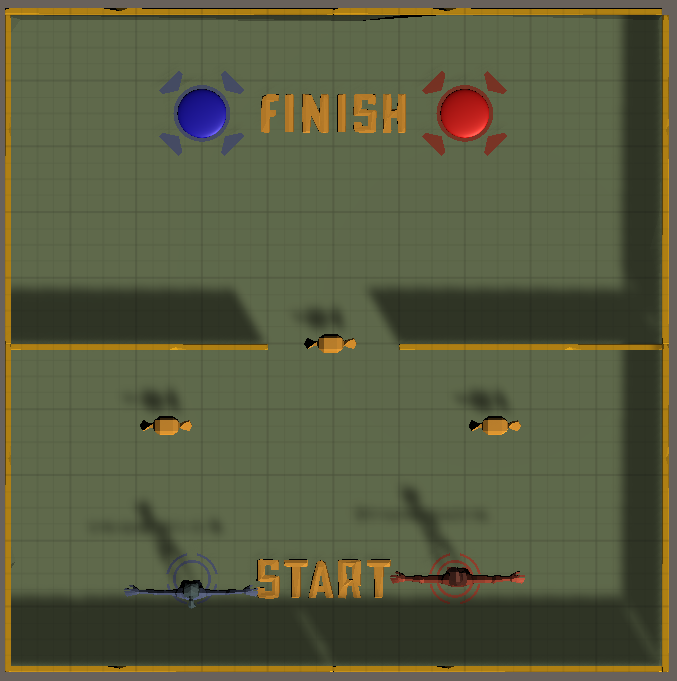
\includegraphics[width=\linewidth]{images/level_1.png}
        \caption{Level 1}
        \label{fig:level 1}
      \end{subfigure}
    \begin{subfigure}[b]{0.45\linewidth}
        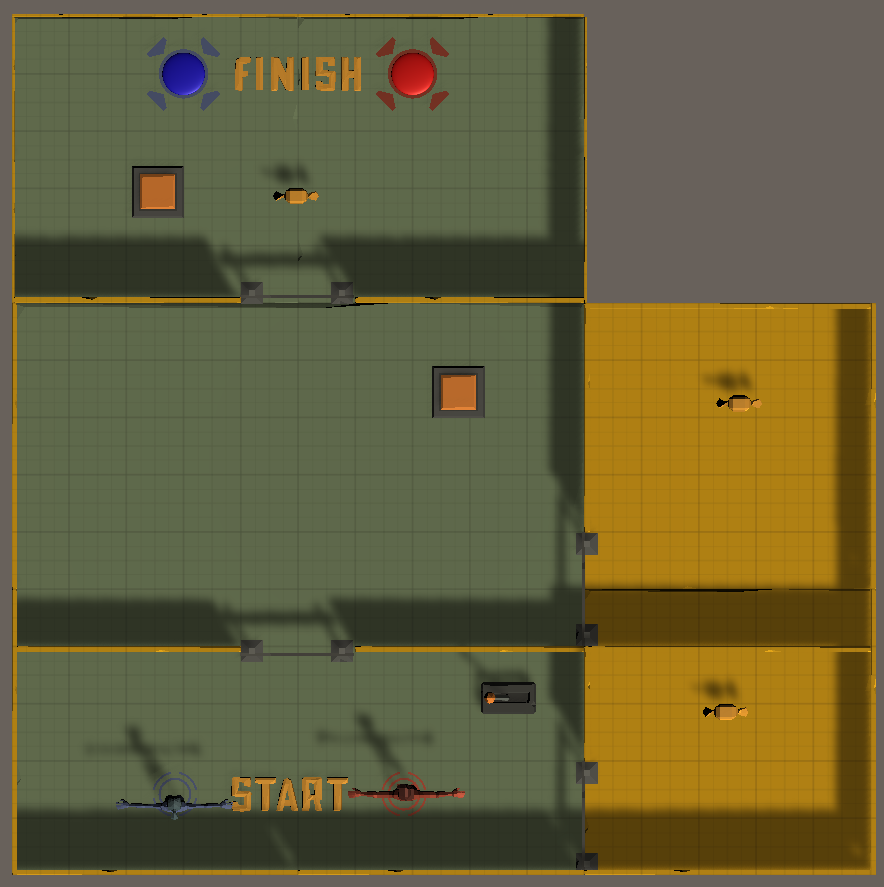
\includegraphics[width=\linewidth]{images/level_3.png}
        \caption{Level 3}
        \label{fig:level 3}
      \end{subfigure}
    \begin{subfigure}[b]{0.45\linewidth}
        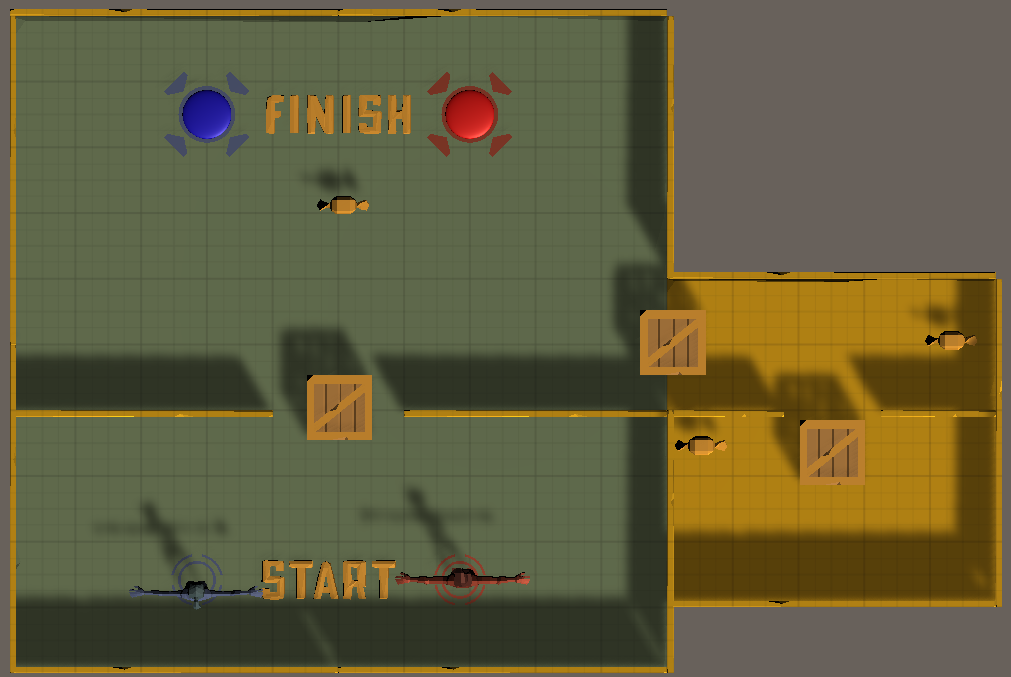
\includegraphics[width=\linewidth]{images/level_2.png}
        \caption{Level 2}
        \label{fig:level 2}
      \end{subfigure}
    \begin{subfigure}[b]{0.45\linewidth}
        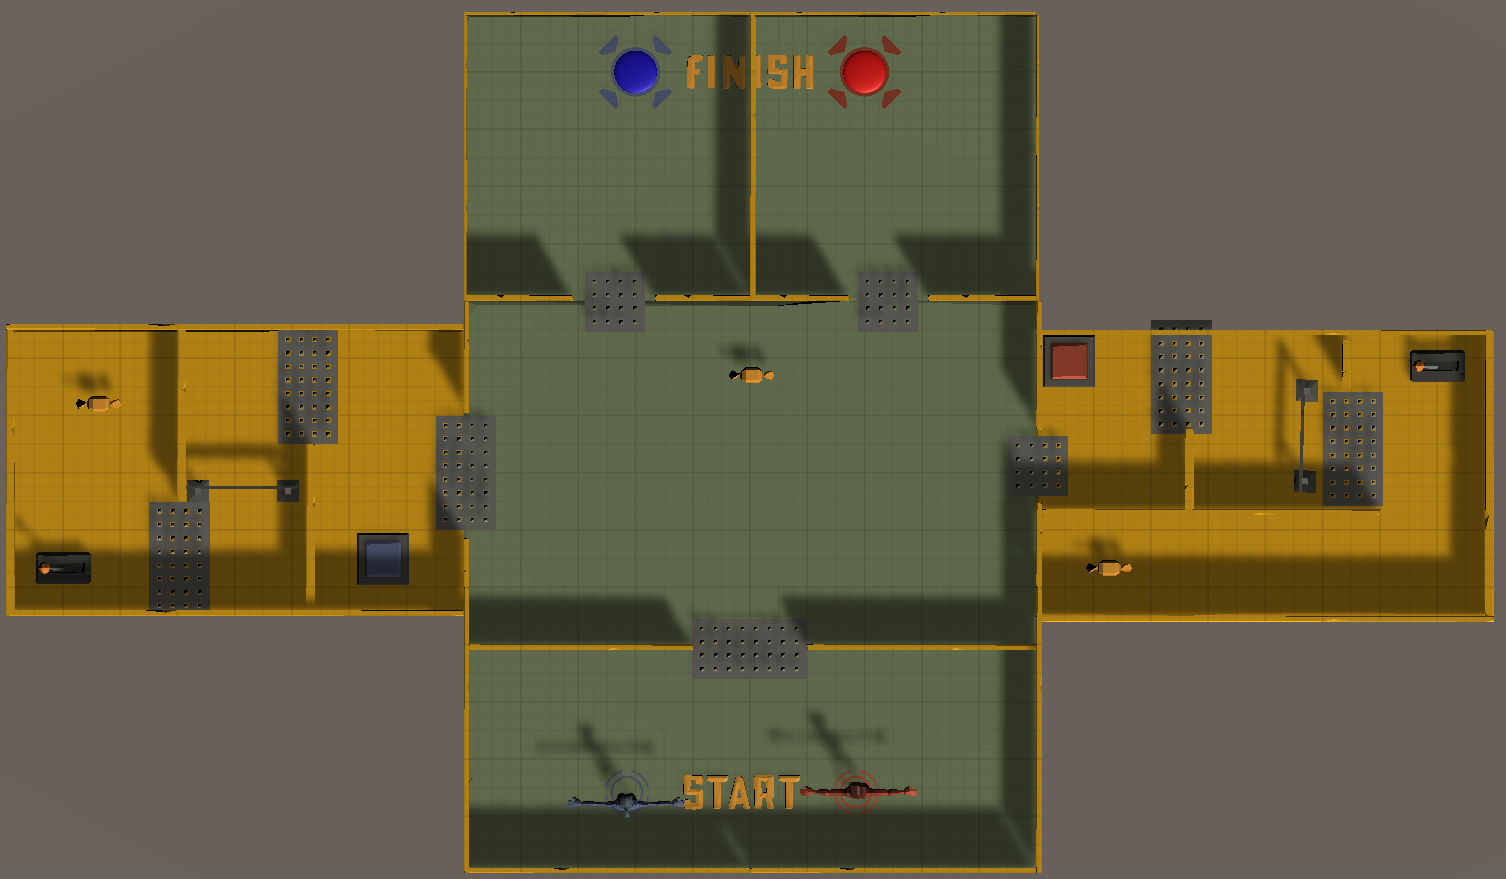
\includegraphics[width=\linewidth]{images/level_4.png}
        \caption{Level 4}
        \label{fig:level 4}
      \end{subfigure}
    \begin{subfigure}[b]{0.45\linewidth}
        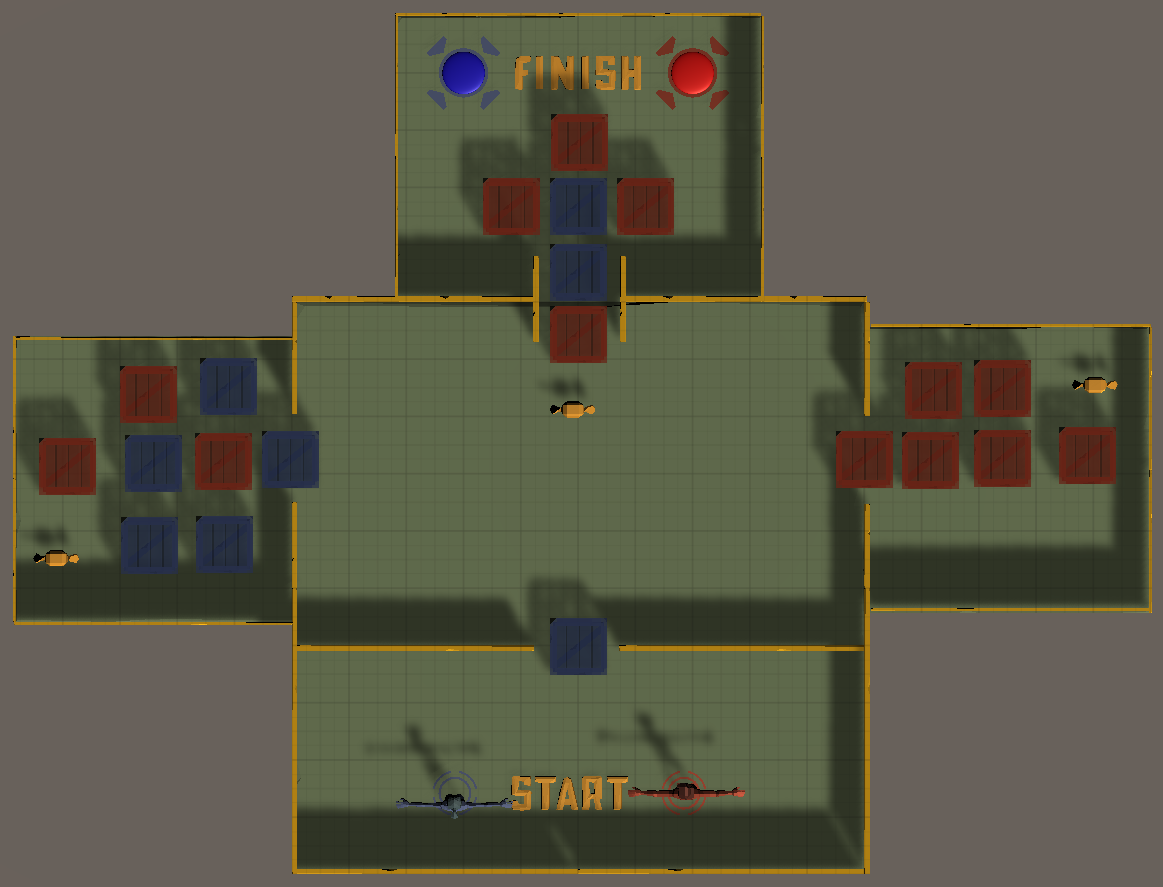
\includegraphics[width=\linewidth]{images/level_5.png}
        \caption{Level 5}
        \label{fig:level 5}
      \end{subfigure}
    \caption{Level 1-5}
\end{figure}


\newpage
\begin{figure}[h!]
    \centering    
    \begin{subfigure}[b]{0.45\linewidth}
        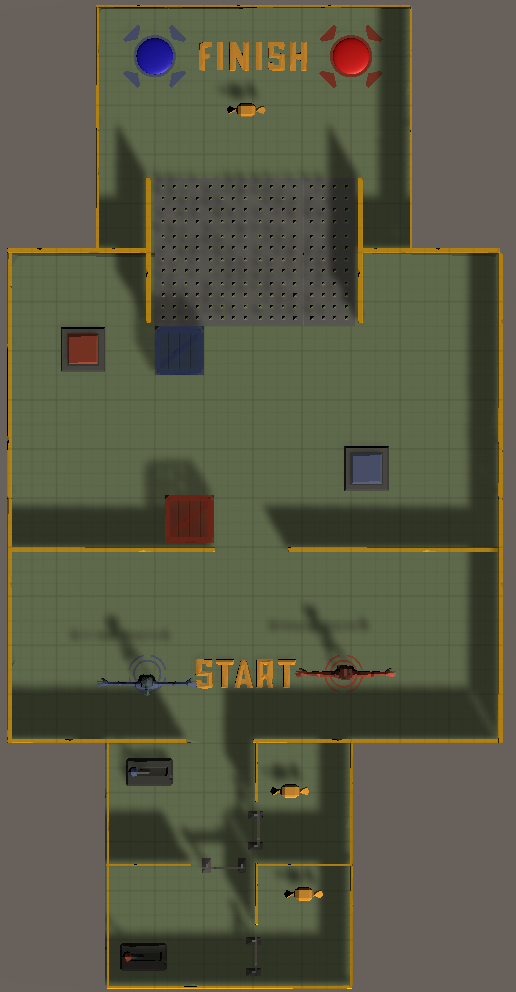
\includegraphics[width=\linewidth]{images/level_6.png}
        \caption{Level 6}
        \label{fig:level 6}
      \end{subfigure}
    \begin{subfigure}[b]{0.45\linewidth}
        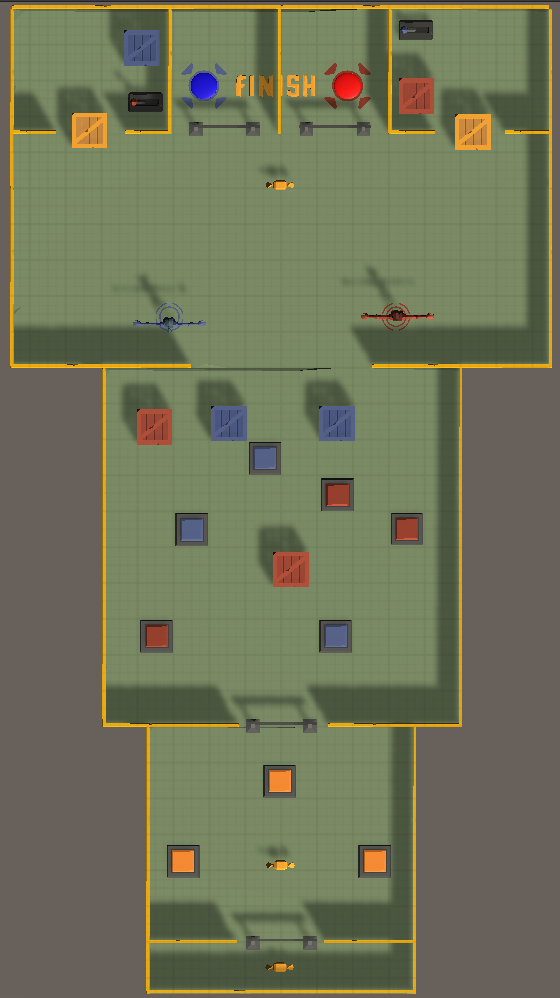
\includegraphics[width=\linewidth]{images/level_8.png}
        \caption{Level 8}
        \label{fig:level 8}
      \end{subfigure}
    \begin{subfigure}[b]{0.45\linewidth}
        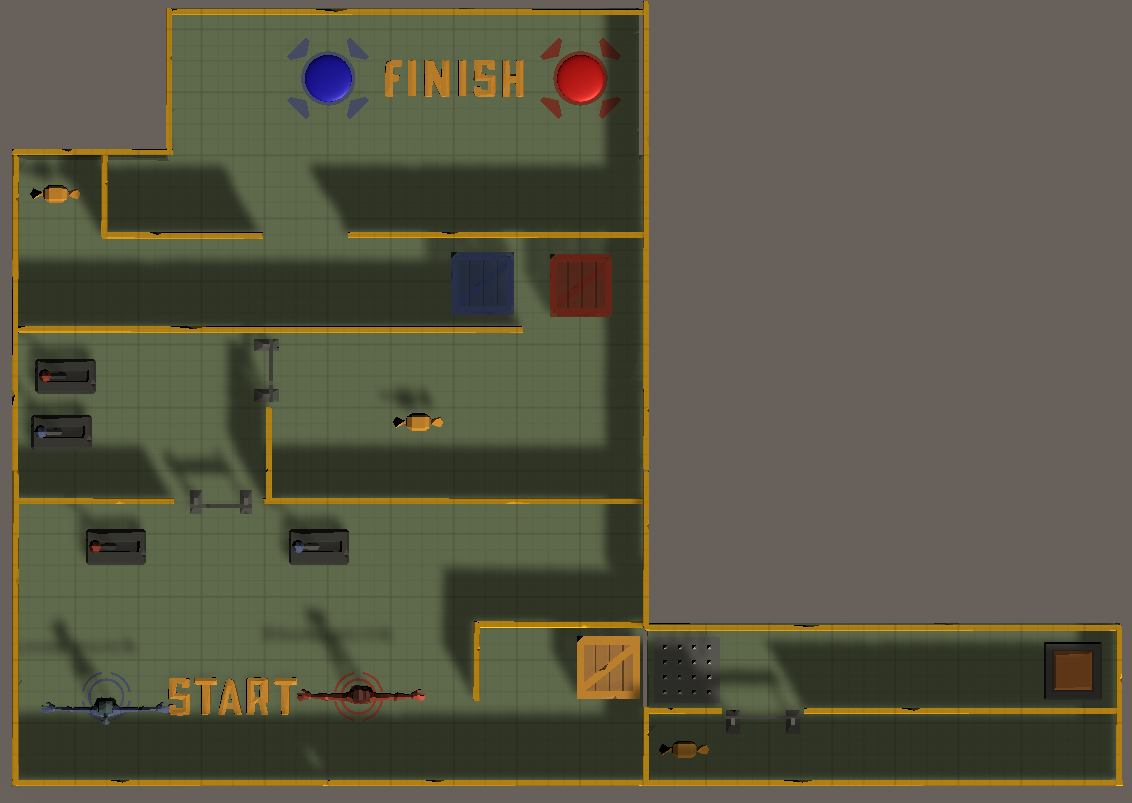
\includegraphics[width=\linewidth]{images/level_7.png}
        \caption{Level 7}
        \label{fig:level 7}
      \end{subfigure}
    \begin{subfigure}[b]{0.45\linewidth}
        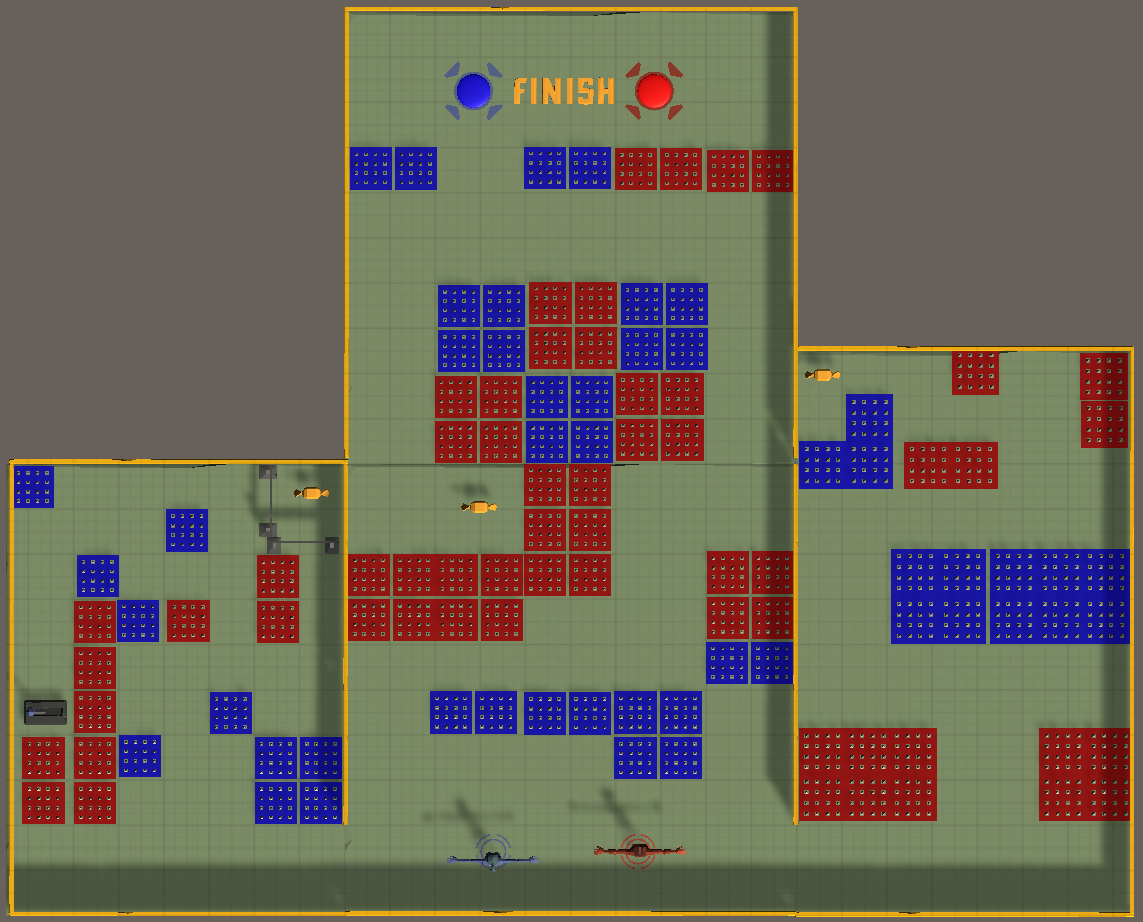
\includegraphics[width=\linewidth]{images/level_9.png}
        \caption{Level 9}
        \label{fig:level 9}
      \end{subfigure}
    \caption{Level 6-9}
\end{figure}